\documentclass{article}

\usepackage{fancyhdr}
\usepackage{extramarks}
\usepackage{amsmath}
\usepackage{amsthm}
\usepackage{amssymb}
\usepackage{amsfonts}
\usepackage{tikz}
\usepackage[plain]{algorithm}
\usepackage{algpseudocode}
\usepackage{graphicx,subfigure} 
\usepackage{comment}
\usepackage{listings}
\usepackage{courier}
\usepackage[version=3]{mhchem}
\usepackage{wasysym}
\usepackage{enumitem}
\lstloadlanguages{[5.2]Mathematica}
\lstset{basicstyle=\footnotesize\ttfamily}

\usetikzlibrary{automata,positioning}

%
% Basic Document Settings
%

\topmargin=-0.45in
\evensidemargin=0in
\oddsidemargin=0in
\textwidth=6.5in
\textheight=9.0in
\headsep=0.25in

\linespread{1.1}

\pagestyle{fancy}
\chead{\hmwkClass\ (\hmwkClassInstructor,\ \hmwkClassTime): \hmwkTitle}
\lhead{\firstxmark}
\rhead{\hmwkAuthorName}
\lfoot{\lastxmark}
\cfoot{\thepage}

\renewcommand\headrulewidth{0.4pt}
\renewcommand\footrulewidth{0.4pt}

\setlength\parindent{0pt}

%
% Create Problem Sections
%

\newcommand{\enterProblemHeader}[1]{
    \nobreak\extramarks{}{Problem \arabic{#1} continued on next page\ldots}\nobreak{}
    \nobreak\extramarks{Problem \arabic{#1} (continued)}{Problem \arabic{#1} continued on next page\ldots}\nobreak{}
}

\newcommand{\exitProblemHeader}[1]{
    \nobreak\extramarks{Problem \arabic{#1} (continued)}{Problem \arabic{#1} continued on next page\ldots}\nobreak{}
    \stepcounter{#1}
    \nobreak\extramarks{Problem \arabic{#1}}{}\nobreak{}
}



%
% Homework Problem Environment
%
% This environment takes an optional argument. When given, it will adjust the
% problem counter. This is useful fo when the problems given for your
% assignment aren't sequential. See the last 3 problems of this template for an
% example.
%
\newenvironment{homeworkProblem}[1][-1]{
    \ifnum#1>0
        \setcounter{homeworkProblemCounter}{#1}
    \fi
    \section{Problem \arabic{homeworkProblemCounter}}
    \setcounter{partCounter}{1}
    \enterProblemHeader{homeworkProblemCounter}
}{
    \exitProblemHeader{homeworkProblemCounter}
}

%
% Homework Details
%   - Title
%   - Due date
%   - Class
%   - Section/Time
%   - Instructor
%   - Author
%

\newcommand{\hmwkTitle}{Mini-Project}
\newcommand{\hmwkDueDate}{Friday, Nov. 5, 2016 at 6:00pm}
\newcommand{\hmwkClass}{CS 187}
\newcommand{\hmwkClassTime}{Section 1}
\newcommand{\hmwkClassInstructor}{Prof. Perona}
\newcommand{\hmwkAuthorName}{Albert Ge }

%
% Title Page
%

\title{
    \vspace{2in}
    \textmd{\textbf{\hmwkClass:\ \hmwkTitle}}\\
    \normalsize\vspace{0.1in}\small{Due\ on\ \hmwkDueDate}\\
    \vspace{0.1in}\large{\textit{\hmwkClassInstructor,\ \hmwkClassTime}}
    \vspace{3in}
}

\author{\textbf{\hmwkAuthorName} }
\date{}

\renewcommand{\part}[1]{\textbf{\large Part \Alph{partCounter}}\stepcounter{partCounter}\\}


%
% Various Helper Commands
%

% Useful for algorithms
\newcommand{\alg}[1]{\textsc{\bfseries \footnotesize #1}}

% For derivatives
\newcommand{\deriv}[1]{\frac{\mathrm{d}}{\mathrm{d}x} (#1)}

% For partial derivatives
\newcommand{\pderiv}[2]{\frac{\partial}{\partial #1} (#2)}

% Integral dx
\newcommand{\dx}{\mathrm{d}x}

% Alias for the Solution section header
\newcommand{\solution}{\textbf{\large Solution}}

% Probability commands: Expectation, Variance, Covariance, Bias
\newcommand{\E}{\mathrm{E}}
\newcommand{\Var}{\mathrm{Var}}
\newcommand{\Cov}{\mathrm{Cov}}
\newcommand{\Bias}{\mathrm{Bias}}

\begin{document}

\maketitle

\pagebreak

\section{Introduction}
So far in class, much attention has been devoted to the transition of the biology of neurons into computational machines that simulate the concept of learning. From understanding how neurons carry electrical signals and developing models for decision boundaries, we have developed a holistic approach to the foundations of neural computation, and showed proof-of-concepts for how one might learn on given data. \\
However, neural computation has come a long way since being just a prototype. Neural networks have recently become an extensively researched topic, with promising modern applications. In that time, neural computation has received a variety of techniques and tools to help make learning more practically feasible and useful. In this mini-project we explore a few ways that researchers have discovered to make machine learning more efficient and accurate: in regularization, convolutional neural networks, and different activation layers. 

\section{Regularization}
Regularization works well then there is huge variability in the classification. This may be due to a poor choice of hypotheses with which to fit the data, or perhaps when the network is already prebiased. \\
Consider an example where the initialization of weights of the network are biased towards positive values only.
Without much additional bells and whistles, this neural network is poor at classifying images of digits. A neural network was trained with three hidden layers each with 30 units (Figure \ref{fig:net1}), and all weights were randomly initialized between 0 and 1). The neural net was trained for 20 epochs on 10000 training images, using RMSprop optimization to speed up convergence time, and tested with 10000 test images. The scores for accuracy and classification error are not very good, just barely above random classification:
\begin{table}[H]
    \caption{Classification Scores without Regularization}
    \centering

    \begin{tabular}{|c|c|}
    \hline

    \hline
    \textbf{Mean squared classification error } & \textbf{Test data accuracy} \\
    \hline
        0.5738 &  0.1135 \\
    \hline
    \end{tabular}
\end{table}

A potential upgrade to the neural net is to introduce regularization to the weights. In brief, regularization is essentially introducing an additional term, dependent on the size of the weights, in the loss function; intuitively, it favors small weight values, and this reduces the overall variance of classification and prevent overfitting. In this section both L1 and L2 regularization are used to see if the classification rate can be improved. 


\begin{figure}[H]
    \centering
    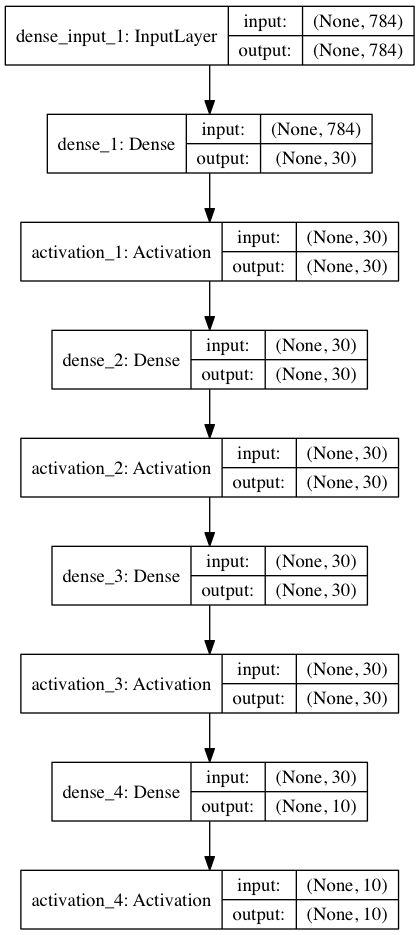
\includegraphics[width=5cm]{model}
    \caption{Schematic of the neural network to be used for regularization experiments. All experiments used the MNIST data set, and classified the images into one of ten different digits. There are a total of five layers; the input, consisting of 784 units, three hidden layers, each with 30 units, and the output layer, consisting of ten units.}
    \label{fig:net1}
\end{figure}

\subsection{L2 Regularization}
The cost function for L2 regularization can be given by:
\[
    C = \mathcal{L} + \frac{1}{N} \sum_w \lambda |w^2|
\] 
where $\mathcal{L}$ is the loss function, $N$ the number of samples, $\lambda$ a free parameter, and $w$ contains the weights of the network. The network is trained by minimizing the cost function for all weights, and performs this optimization problem by taking the gradient of the cost with respect to the weights. \\

To understand how to effectively use L2 regularization for classifiying MNIST, an experiment was conducted by varying the free parameter, $\lambda$, and observing the resulting classification rate. Figure \ref{fig:mse2} shows the results of this experiment. \\


\begin{figure}[H]
    \centering
    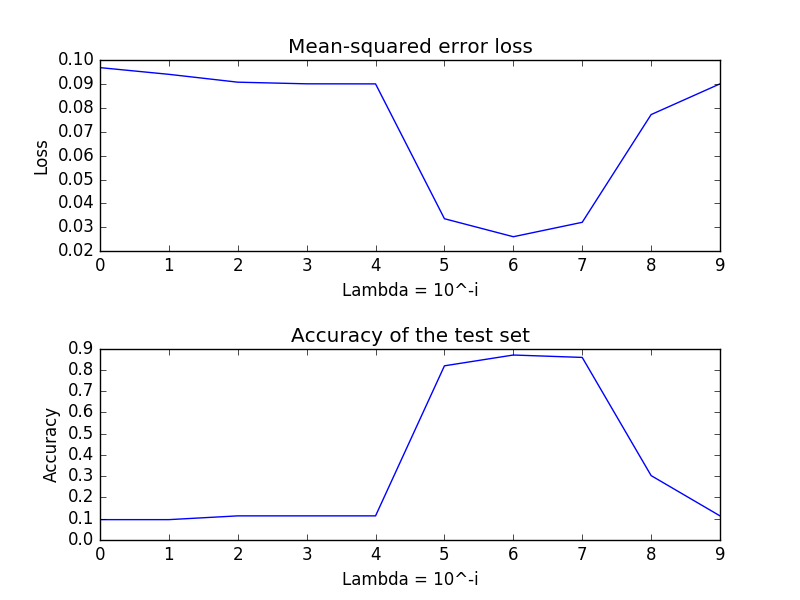
\includegraphics[width=10cm]{mse.png}
    \caption{Mean-squared error and accuracy over the test set for L2 regularization. Optimal MSE is about 0.0261, and optimal accuracy is 0.87, for $\lambda = 10^{-6}$.}
    \label{fig:mse2}
\end{figure}

For small values of $\lambda$, the regularization appears to contribute very well to the classification rate. For values of $\lambda \geq 10^{-4}$, however, the accuracy plummets back to random classification rates. A possible explanation of this is underfitting; the weight values are being pushed down enough such that nothing in the test data can be classified well. A further analysis shows that too small values of $\lambda < 10^{-7}$ also do not fit the data well; for brevity, these plots are excluded. Figure \ref{fig:L2} shows this phenomena clearly; for each value of $\lambda$ the weight matrix between the first and second hidden layer was plotted as a heatmap. 


\begin{figure}[H]
\centering
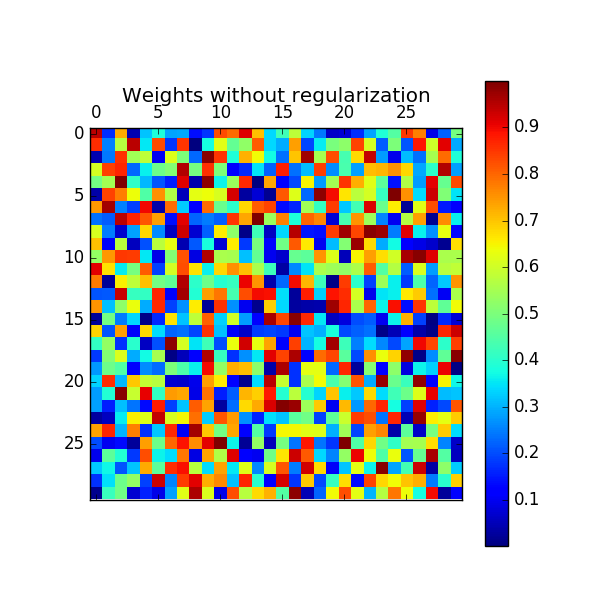
\includegraphics[width=45mm]{no_reg}
\subfigure{\label{fig:0}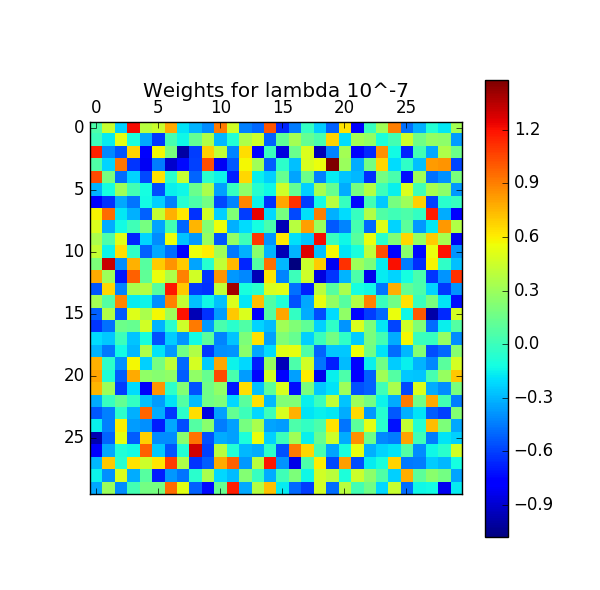
\includegraphics[width=45mm]{lambda7.png}}
\subfigure{\label{fig:1}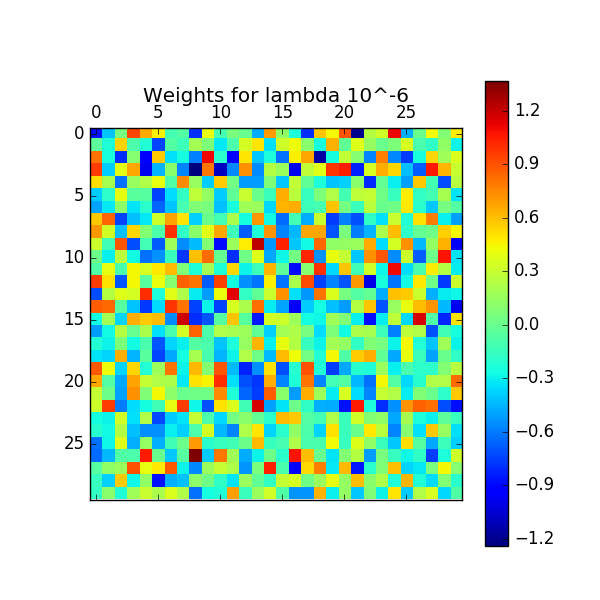
\includegraphics[width=45mm]{lambda6.png}}
\subfigure{\label{fig:2}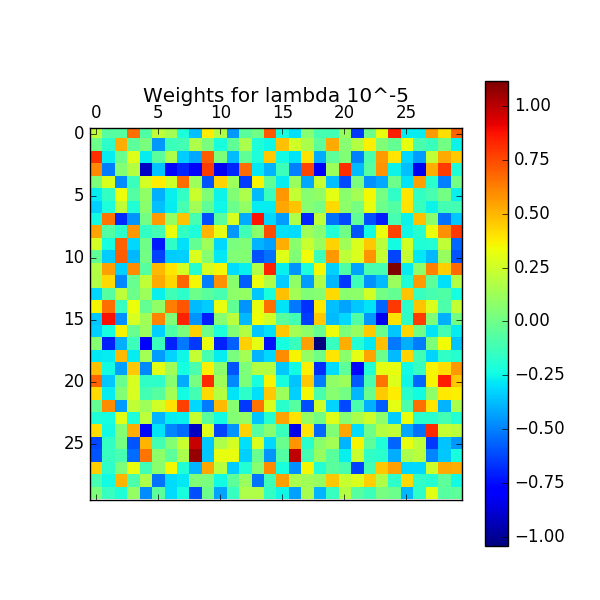
\includegraphics[width=45mm]{lambda5.png}}
\subfigure{\label{fig:3}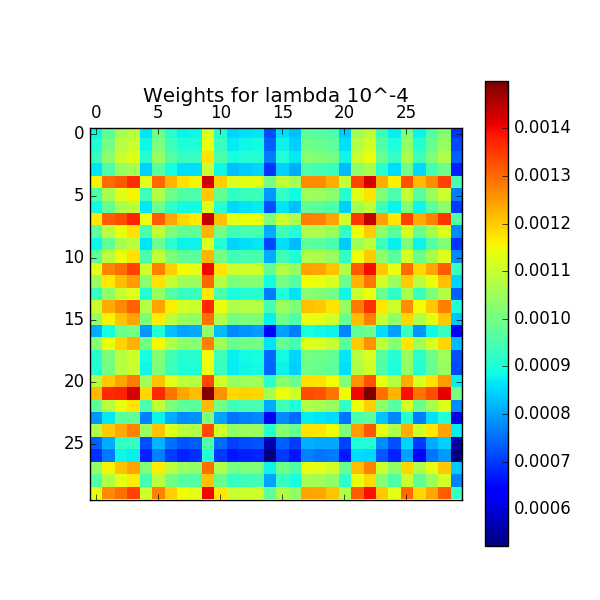
\includegraphics[width=45mm]{lambda4.png}}
\subfigure{\label{fig:4}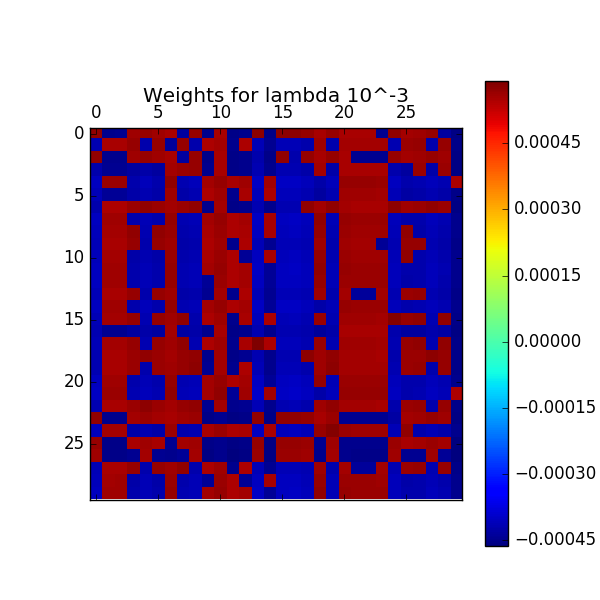
\includegraphics[width=45mm]{lambda3.png}}
\subfigure{\label{fig:5}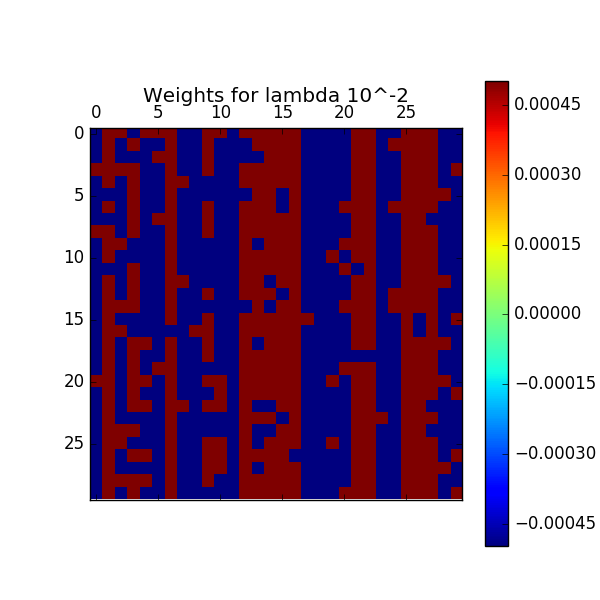
\includegraphics[width=45mm]{lambda2.png}}
\subfigure{\label{fig:6}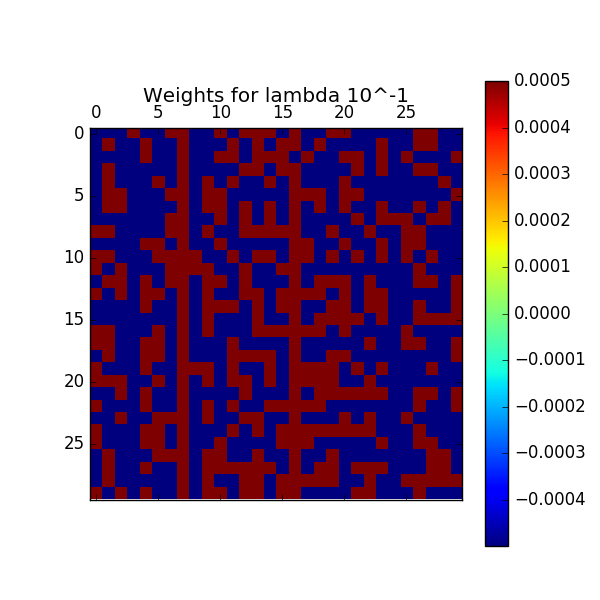
\includegraphics[width=45mm]{lambda1.png}}
\subfigure{\label{fig:7}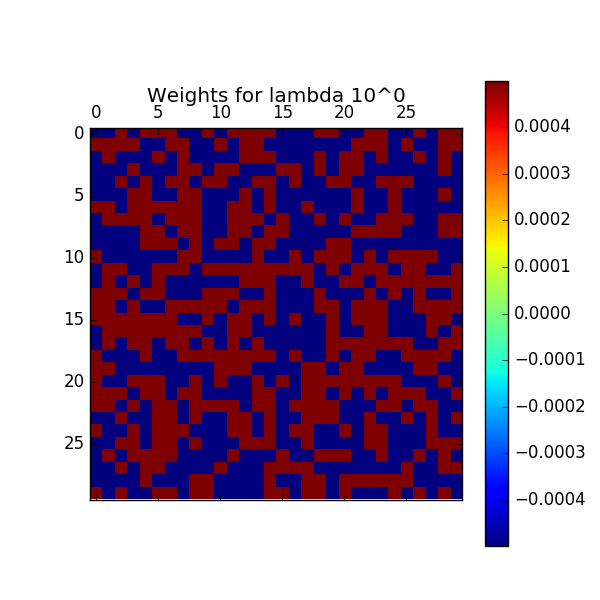
\includegraphics[width=45mm]{lambda0.png}}
\caption{Heatmap of weight matrices for the second layer (L1) in the neural network. Each heatmap is generated using the final weights used to train the neural net, and for varying degrees of regularization.}
\label{fig:L2}
\end{figure}

As $\lambda$ increases, the weights are being pushed down, but there appears a dichotomy of weights; either close to the max values, or close to the min values. This dichotomization suggests the limitation in too much regularization; it cannot capture subtleties of the data as well with only a few weight values, so classification is poor.

\subsection{L1 regularization}
The cost function for L2 regularization can be given by:
\[
    C = \mathcal{L} + \frac{1}{N} \sum_w \lambda |w|
\] 
The same series of experiments were run, varying the value of $\lambda$, and plotting the accuracy and weight matrices of each network:

\begin{figure}[H]
    \centering
    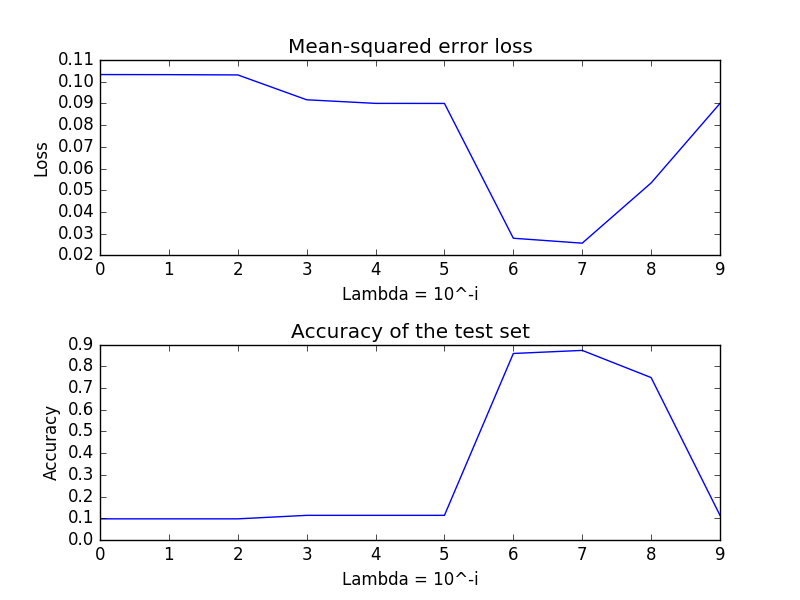
\includegraphics[width=10cm]{mse1.png}
    \caption{Mean-squared error and accuracy over the test set for L1 regularization. Optimal MSE is about 0.0256, and optimal accuracy is 0.87, for $\lambda = 10^{-7}$.}
    \label{fig:mse1}
\end{figure}


\begin{figure}[H]
\centering
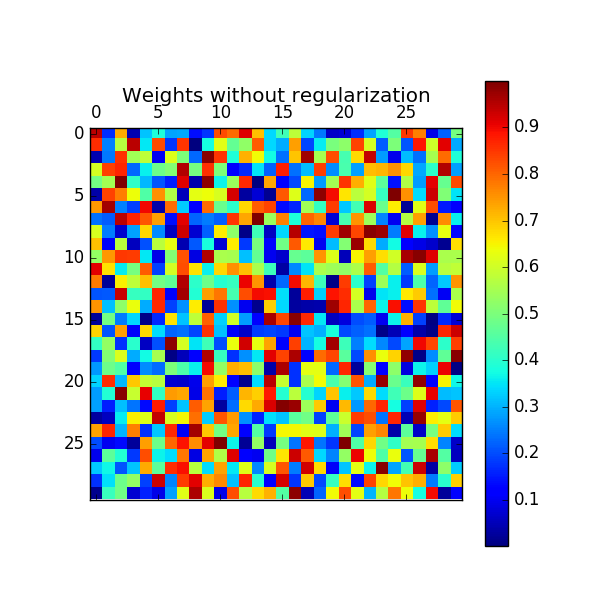
\includegraphics[width=45mm]{no_reg}
\subfigure{\label{fig:10}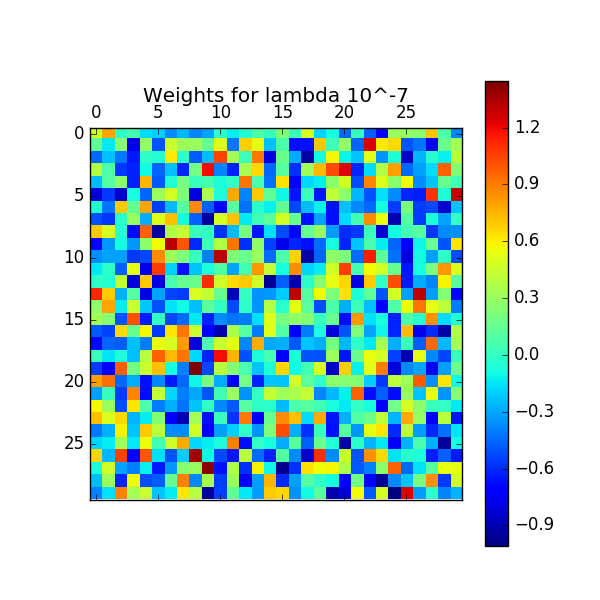
\includegraphics[width=45mm]{lambda17.png}}
\subfigure{\label{fig:11}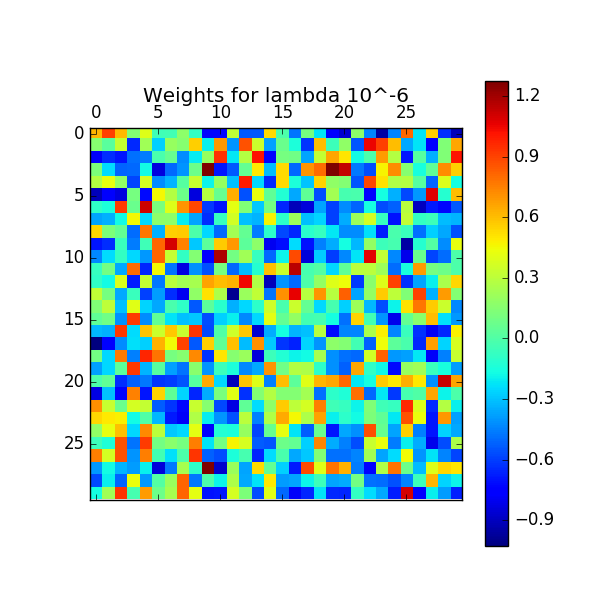
\includegraphics[width=45mm]{lambda16.png}}
\subfigure{\label{fig:12}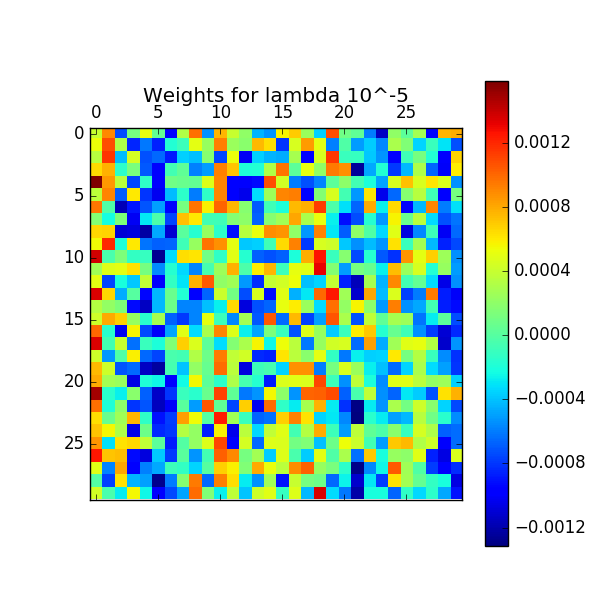
\includegraphics[width=45mm]{lambda15.png}}
\subfigure{\label{fig:13}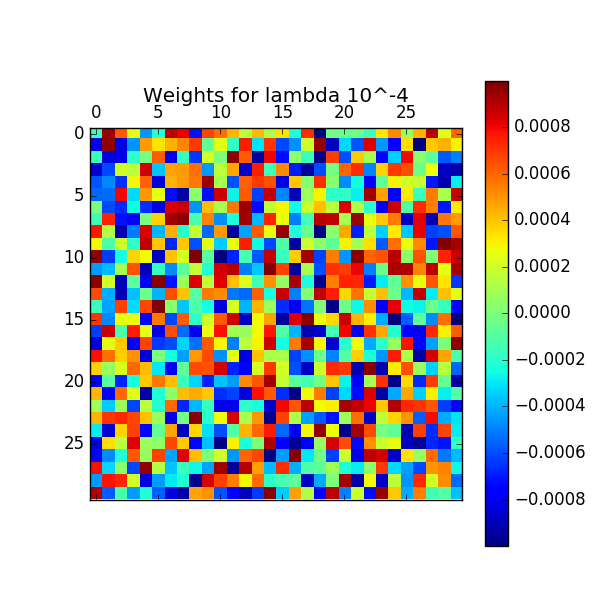
\includegraphics[width=45mm]{lambda14.png}}
\subfigure{\label{fig:14}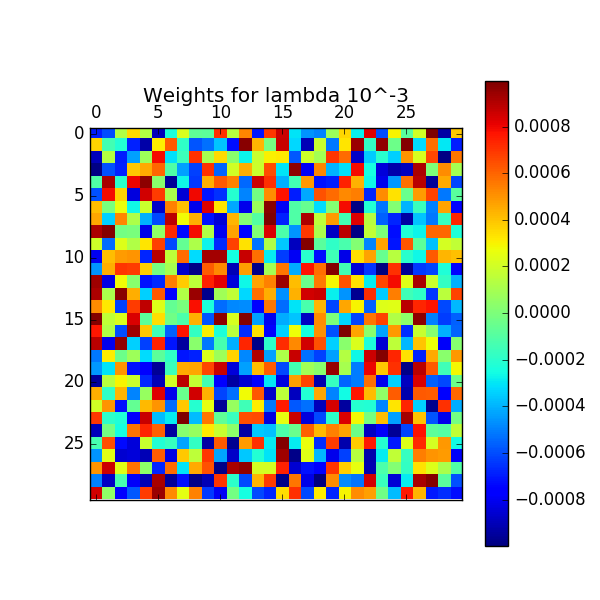
\includegraphics[width=45mm]{lambda13.png}}
\subfigure{\label{fig:15}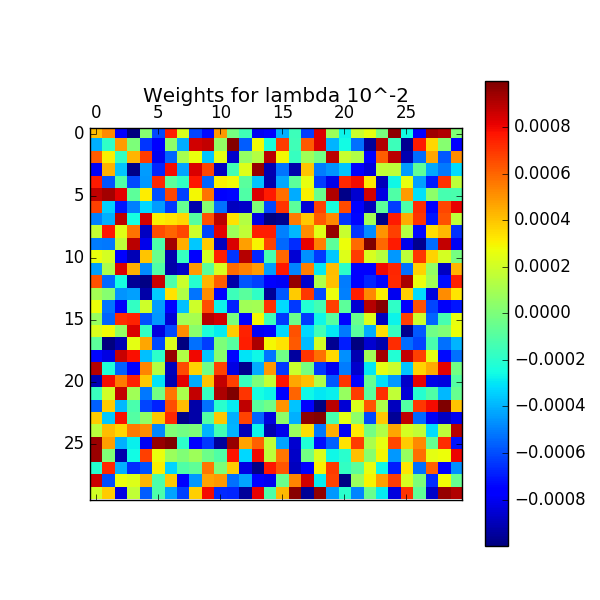
\includegraphics[width=45mm]{lambda12.png}}
\subfigure{\label{fig:16}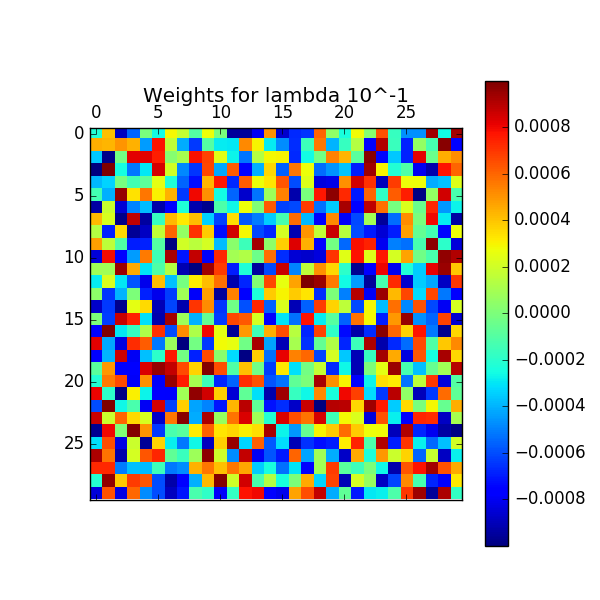
\includegraphics[width=45mm]{lambda11.png}}
\subfigure{\label{fig:17}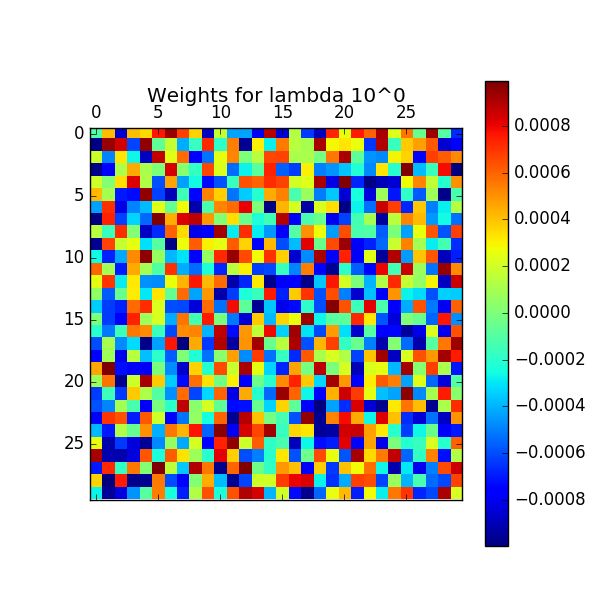
\includegraphics[width=45mm]{lambda10.png}}
\caption{Heatmap of weight matrices for the second layer (L1) in the neural network. Each heatmap is generated using the final weights used to train the neural net, and for varying degrees of regularization.}
\label{fig:L1}
\end{figure}

The effect of L1 regularization is similar; for particular small values of $\lambda$ the classification rate skyrockets, and is low otherwise. Classification on the testing set remains similar for both L1 and L2. L1 regularization also decreases the absolute value of weights of the network; however, the same dichotomization in L2 is not observed in L1 regularization. It that many more weights are closer to zero in value, suggesting a sparse matrix.  \\
In conclusion, regularization is able to correct for prebiased weights, helping achieve optimal accuracy in a shorter amount of time.

\section{Convolutional Neural Networks}
Regularization has demonstrated that accuracy of classification can improve to about 90\%; but can it be done better? A popular tool used today learning specifically on image sets uses a concept known as convolutional neural network. A convolutional neural network can be thought of as learning on two-dimensional patterns in the image. This takes advantage of the two-dimensionality of an image set; as opposed to a multi-layer perceptron, which simply maps all the image's pixels into a single vector, thereby losing information about adjacent pixels, a convolutional neural network can look for relative positions of patterns and use those to make decisions about how the patterns are important to each other. \\
The patterns that the network is looking for are called filters. Intuitively, the filters are "overlayed" over portions of the image, and the underlying image can "fit" the filter (if multipliying element-wise the pixel values and seeing if the dot product result is positive). By convolving (iterating) through all continguous blocks of the image, a matrix, consisting of these dot product values, can be formed, known as a feature map. This feature map can then be trained as in a multi-layer perception, with threshold units and weights. Finally, to reduce the overall complexity of the network and lower the risk of overfitting, these features can be aggregated to produce a smaller number of disjoint "pools", so that only the most prominent features are filtered through the convolution.\\

This section compares the performance of convolution neural networks and multi-layer perceptrons. For the multi-layer perceptrons, a network architecture of one hidden layer with 30 units is used, as in Figure \ref{fig:MLP}. For convolutional neural networks, the same 30-unit hidden layer is stacked atop two convolutional layers, which apply 32 filters of 3 pixels by 3 pixels to the image data, and a pooling layer, split into 2 by 2 disjoint pools. This architecture is shown in Figure \ref{fig:CNN}. In between each convolution layer a tanh activation layer was used. Both networks were trained on 10000 training images for ten epochs, and tested on 10000 testing images.

\begin{figure}[H]
    \centering
    % 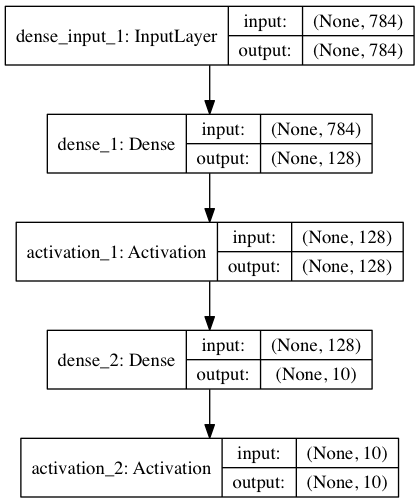
\includegraphics[width=5cm]{modelMLP}
    \subfigure[Multi-layer Perceptron]{\label{fig:MLP}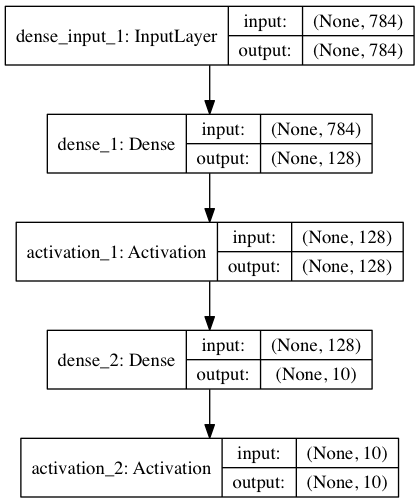
\includegraphics[width=5cm]{modelMLP.png}}
    \subfigure[Convolutional Neural Network]{\label{fig:CNN}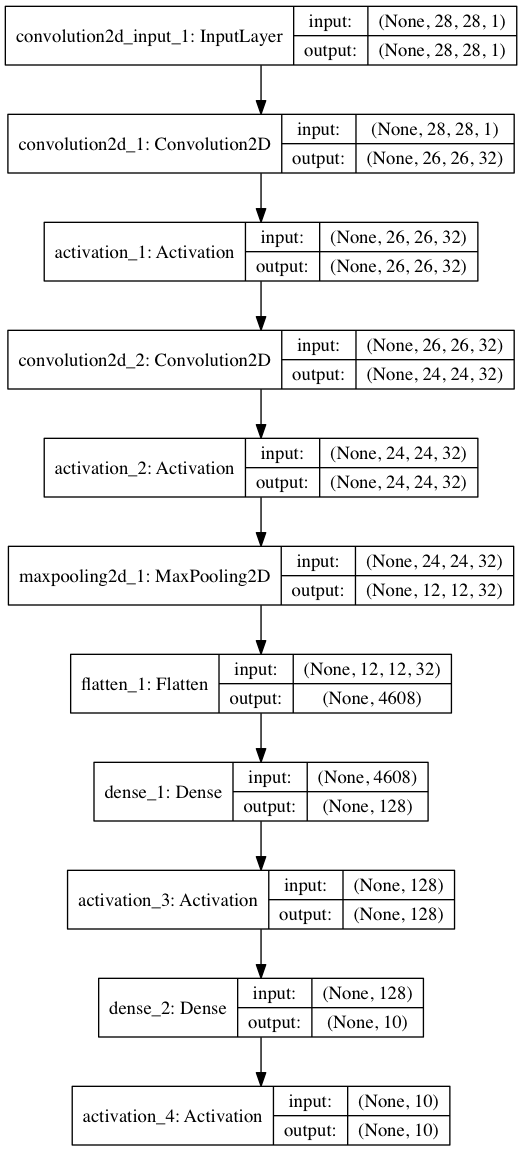
\includegraphics[width=5cm]{modelCNN.png}}
    \caption{Network architecture for neural networks training on MNIST}
\end{figure}

\begin{figure}[H]
    \centering
    % 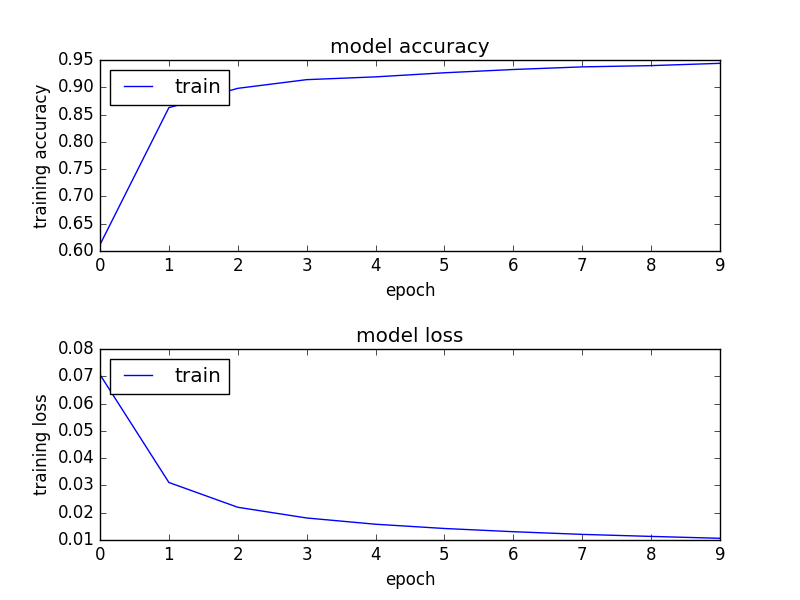
\includegraphics[width=10cm]{mnist_mlp}
    \subfigure[Multi-layer Perceptron]{\label{fig:mlp2}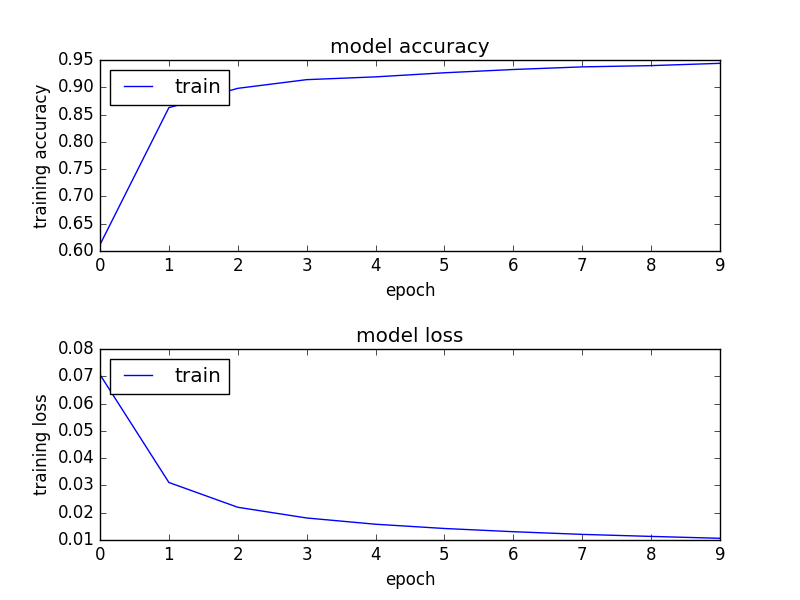
\includegraphics[width=8cm]{mnist_mlp}}
    \subfigure[Convolutional Neural Network]{\label{fig:cnn2}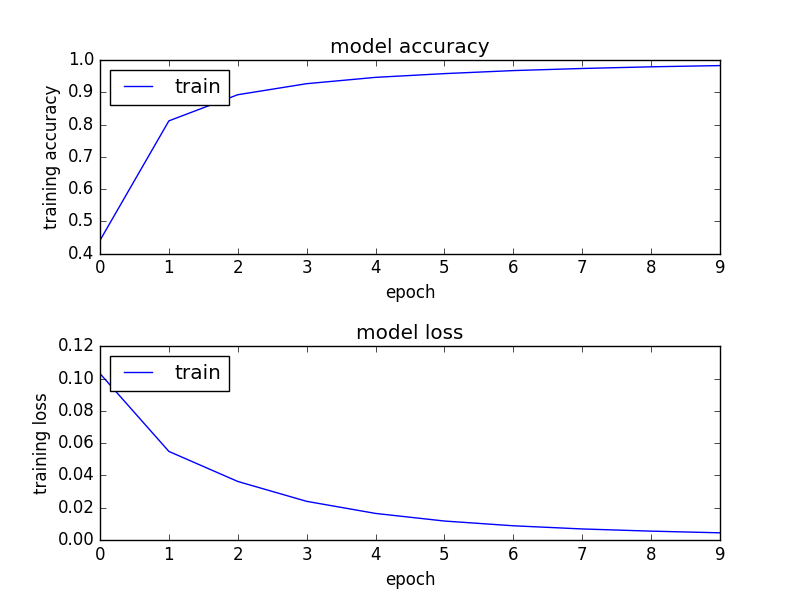
\includegraphics[width=8cm]{mnist_CNN.png}}
    \caption{Loss and accuracy as a function of number of epochs. For the perceptron, final loss was 0.0175, and test accuracy was 0.9083. For the convolutional neural network, final loss was 0.0045, and test accuracy was 0.9827.}
\end{figure}
Convolutional neural networks, while much longer to compute, achieve a much higher test accuracy rate. Thus, convolutional neural networks show how to improve beyond the 90\% accuracy plateau.


\section{Activation Layers}

A final consideration is the different nonlinear functions used in activation layers. Throughout the project, much experimentation was done on determining the parameters that would determine optimal classification performance. In doing so, it was discovered that different nonlinear functions also significantly affects classification. This naturally led to the question of exploring the behavior of different nonlinearities and observing their affect on the output. \\
For most experiments, the sigmoid nonlinearity was used as an activation layer. Recall that the sigmoid function is defined as the following:
\[
        S(t) = \frac{1}{1 + e^{-t}}
\]
Thus, inputs are mapped to between 0 and 1. As already shown in Figure \ref{fig:mlp2}, the architecture in Figure \ref{fig:MLP}, and only sigmoid for the activation layer yields a test accuracy of about 90\%.\\

Here we test a variety of available activation layers in the Keras deep learning library using the exact same architecture, training and testing images, and only changing the type of activation layer, and record their final loss and accuracy values. A full suite of nonlinearities are given in Table \ref{tab:nonlinear}, but for brevity only the tanh and relu functions will be discussed. \\

Relu, or known as the rectifier linear unit, maps inputs to strictly nonnegative values. It is just defined as 
\[
    f(t) = max(0, t)
\]
The rectifier affords a number of advantages in the computation of a multi-layer perceptron's weights. For example, it does not experience the vanishing gradient problem, which occurs multiplying weights by small values. This subsequently decreases the magnitude of the gradient, and causes networks to train very slowly, as the weights will not change much with small gradient values. As seen in the table, the relu activation actually has slightly better classification on the 10000 test images over sigmoid, with about 93\% classification. \\
Tanh, the hyperbolic tangent function, performs equally as well as, if not better than, the sigmoid function, with a classification of 90\% as well. One important distinction is that tanh maps inputs from -1 to 1. This reduces biasing the gradients towards one direction, since sigmoid maps inputs from 0 to 1, and so the gradient would always stay the same sign. 
\begin{table}[H]
    \label{tab:nonlinear}
    \centering

    \begin{tabular}{|l|c|c|c|}
    \hline

    \hline
    \textbf{Name} & \textbf{Mean-squared error Loss} & \textbf{Accuracy} \\
    \hline
    Softmax & 0.0396 & 0.843  \\
    \hline
    Softplus & 0.0209 & 0.92 \\
    \hline
    Softsign & 0.0354 & 0.900 \\
    \hline
    Relu (Rectifier) & 0.015 & 0.934 \\
    \hline
    Tanh & 0.0267 & 0.9083 \\
    \hline
    Sigmoid & 0.018 & 0.907 \\
    \hline
    Hard Sigmoid & 0.017 & 0.906 \\
    \hline
    Linear & 0.044 & 0.823 \\
    \hline
    \end{tabular}
    \caption{Effect of nonlinear activations on MNIST classification. Best-performing activation layer was relu, and worst-performing activation layer was linear.}
\end{table}

The advantages afforded by different nonlinearities suggest that one must be careful in choosing the right activation layer for their network.


\section{Conclusion}
This miniproject delved into modern techniques used in neural networks to improve the accuracy for a practically relevant application - classifying images of digits. The topics of L1/L2 regularization, convolutional neural networks, and nonlinear activations were investigated, each revealing how the accuracy of classifying MNIST could be improved by adding features to a vanilla implementation of a multi-layered neural network. Moreover, these topics have demonstrated the wide field that is neural computation, and how there is still much to be explored in making neural networks more practically feasible and relied on as a model for automated learning.

\end{document}
